\documentclass[11pt, oneside]{article}   	% use "amsart" instead of "article" for AMSLaTeX format
\usepackage{geometry}                		% See geometry.pdf to learn the layout options. There are lots.
\geometry{letterpaper}                   		% ... or a4paper or a5paper or ... 
%\geometry{landscape}                		% Activate for rotated page geometry
%\usepackage[parfill]{parskip}    		% Activate to begin paragraphs with an empty line rather than an indent
\usepackage{graphicx}				% Use pdf, png, jpg, or eps§ with pdflatex; use eps in DVI mode
% TeX will automatically convert eps --> pdf in pdflatex
\usepackage{subcaption}
\usepackage{amssymb}
\usepackage{color}

%SetFonts

%SetFonts


\title{Neutrino cross section measurements using a 3D grid-like neutrino detector, WAGASCI, in the J-PARC neutrino beamline}
\author{The Author}
%\date{}							% Activate to display a given date or no date

\begin{document}
\maketitle
%\section{}
%\subsection{}

\section{Introduction}

The understanding of neutrino-nucleus interactions in the 1 GeV energy region is critical for the success
of accelerator-based neutrino oscillation experiments such as the T2K experiment.
Complicated multi-body effects of nuclei render this understanding difficult.
The T2K near detectors have been measuring these and significant progress has been achieved.
However, the understanding is still limited.
One of the big factors preventing from full understanding is the non-monochromatic
neutrino beam spectrum.
Measurements with different but some overlapping beam spectra would greatly benefit to resolve the contribution
from different neutrino energies.
We, the Wagasci collaboration, proposes to study the neutrino-nucleus interaction
at the B2 floor of the neutrino monitor building, where different neutrino spectra
can be obtained due to the different off-axis position.
Our experimental setup contains 3D grid-structure plastic-scintillator detectors filled with water as the neutrino interaction target
(Wagasci modules), two side- and one downstream- muon range detectors(MRD's).
The 3D grid-structure and side-MRD's allows a measurement of  wider-angle scattering than the T2K off-axis near detector (ND280).
High water to scintillator material ratio enables the measurement of the neutrino interaction on water, which
is highly desired for the T2K experiment because it's far detector, Super-Kamiokande, is composed of water.
The MRD's consist of plastic scintillators and iron plates.
The downstream-MRD, so called the Baby MIND detector, is also work as a magnet and provides the charge identification capability as well as magnetic momentum measurement for high energy muons.
The charge identification is essentially important to select antineutrino events in the antineutrino beam
because contamination of the neutrino events is as high as 30\%.
Most of the detectors has been already constructed.
The Wagasci modules have been commissioned as the J-PARC T59 experiment and the Baby MIND detector was commissioned at the CERN neutrino platform.
Therefore, the collaboration will be ready to proceed to the physics data taking for the T2K beam time in January 2019.
We will provide the cross sections of the charged current neutrino and antineutrino interactions on water
with slightly higher neutrino energy than T2K ND280 with wide angler acceptance.
When combined with ND280 measurements, our measurement would greatly improve the understanding of the neutrino interaction
at around 1 GeV and contribute to reduce one of the most significant uncertainty of the T2K experiment.

\section{Experimental Setup}
Figure. \ref{fig:all_detector} shows a schematic view of the entire set of detectors.
A central detector, Wagasci modules, consists of 3D grid-structure plastic-scintillator detectors filled with water as the neturino interaction target.
They are surrounded by two side- and one downstream- muon range detectors(MRD's)
The MRD's are used to select muon tracks from the charged-current (CC) interactions 
and to reject short tracks caused by neutral particles 
that originate mainly from neutrino interactions in material surrounding the central detector, like the walls of the detector hall,
neutrons and gammas, or neutral-current (NC) interactions.
The muon momentum can be reconstructed from its range inside the detector.
The MRD's consist of plastic scintillators and iron plates.
In addition, eaco of the iron plates of the downstream-MRD, so called the Baby MIND detector, is wound by a coil and
can be magnetized. It provide the charge selection capability.

For all detectors, scintillation light in the scintillator bar is collected and transported to a photodetector with a wavelength shifting fiber (WLS fiber).
The light is read out by a photodetector, Multi-Pixel Photon Counter (MPPC), attached to one end of the WLS fiber.
The signal from the MPPC is read out by the dedicated electronics developed for the test experiment
to enable bunch separation in the beam spill.
The readout electronics is triggered using the beam-timing signal from MR to synchronize to the beam.
The beam-timing signal is branched from those for T2K, and will not cause any effect on the T2K data taking.

\begin{figure}[tbh]
\begin{center}
\includegraphics[width=0.8\linewidth]{fig/all_detector2.pdf}
\end{center}
\caption{
Schematic view of entire sets of detectors.
}
\label{fig:all_detector}
\end{figure}

T2K adopted the off-axis beam method, in which
the neutrino beam is intentionally directed 2.5 degrees away from SK producing a narrowband $\nu_{\mu}$ beam.
The off-axis near detector, ND280, is installed towards the SK direction in the B1 floor of the near detector hall of the J-PARC neutrino beam-line.
We propose to install our detector in the B2 floor of the near detector hall, 
where the off-axis angle is similar but slightly different.
The candidate detector position in the B2 floor is shown in Fig. \ref{fig:location}.
The expected neutrino energy spectrum at the candidate position is shown in Fig. \ref{fig:b2flux}.

\begin{figure}[tbh]
\begin{center}
\includegraphics[width=0.6\linewidth]{fig/location2.pdf}
\end{center}
\caption{
Candidate detector position in the B2 floor of the near detector hall.
}
\label{fig:location}
\end{figure}

\begin{figure}[tbh]
\begin{center}
\includegraphics[width=0.6\linewidth]{fig/fluxes.pdf}
\end{center}
\caption{
Neutrino energy spectrum at the candidate detector position(red).
The spectrum at the ND280 site (black) is also shown.
}
\label{fig:b2flux}
\end{figure}





\subsection{Wagasci module}
The Wagasci module is a neutrino target detector consists of a stainless tank filled with 16 scintillator tracking planes immersed, where each plane is an array of 80 scintillator bars.
The 40 bars, called parallel scintillators, are placed perpendicularly to the beam, and the other 40 bars, called grid scintillators, are placed in parallel to the beam with grid structure.

The dimension of the each Wagasci module is 100cm $\times$ 100cm in the x and y directions
and 50cm along the beam direction.
Thin plastic scintillator bars (thickness $\sim 0.3$cm) are used for the Wagasci module
to reduce  the mass ratio of scintillator bars to water,
because neutrino interactions in the scintillator bars are a background for the cross section measurements.

Inside the Wagasci module, plastic scintillator bars are aligned as a 3D grid-like structure, shown in Fig. \ref{fig:3dgrid}.


Spaces in the 3D grid-like structure are filled with water for the water-in Wagasci module.
The total water mass serving as neutrino targets in the detector are $\sim$0.5 ton.

When neutrinos interact with hydrogen, oxygen or carbon, in water and scintillators,
charged particles are generated.
Neutrino interactions are identified by detecting tracks of charged particles through plastic scintillation bars.
Thanks to the 3 D grid-like structure of the scintillator bars, 
the Wagasci module has $4\pi$ angular acceptance for charged particles.
Furthermore, adopting a 5cm grid spacing, short tracks originated from protons and charged pions can be reconstructed
with high efficiency.

Scintillator bars whose dimensions are 2.5cm x 0.3cm x 100cm are used for the Wagasci module.
The total number of channels in one Wagasci module is 1280.

\begin{figure}[tbhp]
  \begin{center}
   \begin{subfigure}{0.48\textwidth}
     \includegraphics[width=\linewidth]{fig/3d_grid_structure.pdf}
    \end{subfigure}
  \begin{subfigure}{0.48\textwidth}
      \includegraphics[width=\linewidth]{fig/wagasci_mod.pdf}
    \end{subfigure}    
    \end{center}
  \caption{2D track reconstruction efficiency as a function of number of hits (left) and track angle (right).
  Here the track angle is the one reconstructed by the INGRID module.}
\label{fig:wmefficiency}
\end{figure}


\begin{figure}[tbh]
\begin{center}
\includegraphics[width=1.0\linewidth]{fig/3d_grid_structure.pdf}
% \includegraphics[width=0.6\linewidth]{fig/tmp.pdf}
\end{center}
\caption{
Schematic view of 3D grid-like structure of plastic scintillator bars inside the central detector.
}
\label{fig:3dgrid}
\end{figure}

\begin{figure}[tbh]
\begin{center}
\includegraphics[width=0.6\linewidth]{fig/wagasci_mod.pdf}
% \includegraphics[width=0.6\linewidth]{fig/tmp.pdf}
\end{center}
\caption{
Schematic view of Wagasci module.
}
\label{fig:wagasci_mod}
\end{figure}

\begin{figure}[tbh]
\begin{center}
\includegraphics[width=0.8\linewidth]{fig/wagasci_scinti_geometry.pdf}
% \includegraphics[width=0.6\linewidth]{fig/tmp.pdf}
\end{center}
\caption{
Geometry of scintillators used for Wagasci modules.
}
\label{fig:wagasci_scinti_geometry}
\end{figure}


\subsection{Baby MIND}
The Baby MIND is the downstream Muon Range Detector.
It also works as a magnet and provides the charge identification capability
as well as magnetic momentum measurement for high energy muons.

The Baby MIND collaboration \footnote{Contact person: E. Noah, Spokesperson: A. Blondel, Deputy spokesperson: Y. Kudenko} submitted a proposal to the SPSC at CERN, SPSC-P-353.
The project was approved by the CERN research board as Neutrino Platform project NP05 and constructed.
The detector consists of 33 magnet modules, each 3500 mm $\times$ 2000 mm$ \times$ 50 mm (30 mm steel) with a mass of approximately 2 tonnes. Of these magnet modules, 18 are instrumented with plastic scintillator modules. 

%The main Baby MIND systems are the magnet, scintillator and electronics modules \cite{Noah:EPS2017}.
%A total of 3,996 silicon photomultipliers are read out by custom electronics Front End Boards that can process up to 96 channels each, sending charge and timing information of hits in the detector to dedicated data acquisition computers.

%One challenge to be addressed by the Baby MIND collaboration is that of obtaining high charge identification efficiencies for $\mu^+/\mu^-$ down to 500 MeV/c and below. Magnetized iron neutrino detectors are limited by multiple scattering in the iron, and their use is overlooked for applications requiring good charge ID efficiencies below 1 GeV/c. By optimizing the distance between the first magnet modules, rendered possible by the magnet design, our simulations show improved charge identification efficiencies down to 400 MeV/c.


\subsubsection{Magnet modules}

The Baby MIND is built from sheets of iron interleaved with scintillator detector modules but unlike traditional layouts for magnetized iron neutrino detectors (e.g. MINOS) which tend to be monolithic blocks with a unique pitch between consecutive steel segments and large conductor coils threaded around the whole magnet volume, the Baby MIND iron segments are all individually magnetized as shown inf Fig.~\ref{fig:BM_winding}, allowing for far greater flexibility in the setting of the pitch between segments, and in the allowable geometries that these detectors can take. 

The key design outcome is a highly optimized magnetic field map. A double-slit configuration for coil winding was adopted to increase the area over which the magnetic flux lines are homogeneous in $B_x$ across the central tracking region. Simulations show the magnet field map to be very uniform over this central tracking region covering an area of $2800\times2000$ mm$^2$, Fig.~\ref{magnet-cross-sections}. The $B_x$ component dominates in this region, with negligible $B_y$ and $B_z$. This was confirmed by measuring the field with 9 pick-up coils wound around the first module. Subsequent modules were equipped with one pick-up coil. Test results on the 33 modules show all to achieve the required field of 1.5 T for a current of 140 A, with a total power consumption of 11.5 kW. The polarity of the field map shown in Figure \ref{magnet-cross-sections} (middle) can be reversed by changing the power supply configuration.
\insertgraph{0.5}{magnet_assembly_zone.png}{Magnet assembly zone at CERN. }{fig:BM_winding}
\inserttwographs{0.5}{b-field-1500a-280cm-coil.png}{0.4}{magnetic_field_measurements_per_batch.png}{Left) Magnetic field map with a coil along 280 cm of the length of the plate. Right) Measured B field for 33 modules.}{magnet-cross-sections}

\subsubsection{Scintillator modules}
Each of the 18 scintillator modules is constructed from 2 planes of horizontal counters (95 counters in total) and 2 planes of vertical counters (16 counters in total) \cite{Antonova:2017tuf}, arranged with an overlap between planes to achieve close to 100\% hit efficiency for minimum ionizing muons. The arrangement of planes within a module is vertical-horizontal-horizontal-vertical.
The scintillator bars are held in place using structural ladders that align and maintain the counters, Figure \ref{proto-module-ladders}. No glue is used in the process, so counters can be replaced. Aluminum sheets front and back provide light tightness.

\insertthreegraphs{0.32}{top_front_module.png}{0.32}{bottom_front_module.png}{0.32}{rear-half-module.png} {Scintillator modules assembly. Left) top of front half-module showing vertical counters, and the spacers-ladders that set the pitch between horizontal counters and hold them in place. Middle) rear half-module showing horizontal counters on their ladders. Right) Assembled rear half-module, the front half-module can be seen in the background.}{proto-module-ladders}

The plastic scintillator counters were made from 220 mm-wide slabs, consisting of extruded polystyrene doped with 1.5\% paraterphenyl (PTP) and 0.01\% POPOP. They were cut to size then covered with a 30-100 $\mu$m thick diffuse reflector resulting from etching of the surface with a chemical agent \cite{Kudenko:2001qj, Mineev:2011xp}. The horizontal counter size is $2880 \times 31 \times 7.5 $ mm$^3$, with one groove along the length of the bar in which sits a wavelength shifting fiber from Kuraray. The vertical counter size is $1950 \times 210 \times 7.5 $ mm$^3$, with one U-shaped groove along the bar. On each counter, two custom connectors house silicon photomultipliers, MPPC type S12571-025C from Hamamatsu, either side of the horizontal counter, and both connectors at the top for the vertical counter. This geometrical configuration for vertical counters was chosen for ease of connectivity to the electronics, and maintenance operations.

A total of 1744 horizontal counters and 315 vertical counters (including spares) were produced at the Uniplast company (Vladimir, Russia).

\subsubsection{Electronics}
The Baby MIND electronic readout scheme includes several custom-designed boards \cite{Noah:2016ikh}. The revised version is shown in Figure \ref{block_diagrams}. At the heart of the system is the electronics Front End Board (FEB), developed by the University of Geneva. The readout system includes two ancillary boards, the Backplane, and the Master Clock Board (MCB) whose development has been managed by INRNE (Bulgarian Academy of Sciences) collaborators.

%One critical element in the photosensor readout path is the cable bundle, a 5 m extension coaxial cable RG174U that connects the photosensor to the FEB. Each bundle connects up to 32 photosensors. The purpose is to decouple the FEBs from the scintillator modules, which improves accessibility to FEBs and their long term maintainability. The module end of the bundle hosts some electronics that manages the application of the high voltage to the SiPMs, enabling faulty SiPMs to be switched off at that level. This feature was added after the summer 2016 beam tests, where a short circuit on a single channel would disable a bank of 96 channels.

\inserttwographs{0.47}{readout_scheme_2.png}{0.45}{electronics_connectivity_detailed.png}{Left) Baby MIND electronics readout scheme. Right) SiPM-to-FEB connectivity.}{block_diagrams}

The FEBv2 hosts 3 CITIROC chips that can each read in signals from 32 SiPMs \cite{Fleury:2014hfa}. Each signal input is processed by a high gain, and a separate low gain, signal path.
The outputs from the slow shapers can be sampled using one of two modes: a mode with an externally applied delay, and a peak detector mode. A faster shaper can be switched to either HG or LG paths, followed by discriminators with adjustable thresholds providing 32 individual trigger outputs and one OR32 trigger output. An Altera ARIA5 FPGA on the FEBv2 samples these trigger outputs at 400 MHz, recording rising and falling times for the individual triggers and assigning time stamps to these. Time-over-threshold from the difference between falling and rising times gives some measure of signal amplitude, used in addition to charge information and useful if there is more than one hit per bar within the deadtime due to the readout of the multiplexed charge output of $\sim9$ $\mu$s. The ARIA5 also manages the digitization of the sampled CITIROC multiplexed HG and LG outputs via a 12-bit 8-ch ADC. 

%The FEBv2 is designed to fit into a slot in a minicrate as shown in Figure \ref{minicrate}. The front face receives the SiPMs cable bundles, the rear end plugs into the backplane. Up to 6 FEBv2 can be housed in each minicrate. Eight minicrates are distributed either side of the Baby MIND.

The internal 400 MHz clock on the FEBv2 can be synchronized to a common 100 MHz clock. The synchronization subsystem combines input signals from the beam line into a digital synchronization signal (SYNC) and produces a common detector clock (CLK) which can eventually be synchronised to an external experiment clock. Both SYNC and CLK signals are distributed to the FEBs. Tests show the FEB-to-FEB CLK(SYNC) delay difference to be 50 ps (70 ps). Signals from the beam line at WAGASCI include two separate timing signals, arriving 100 ms and 30 $\mu$s before the neutrino beam at the near detectors. The spill number is available as a 16-bit signal. 
%\insertthreegraphs{0.31}{FEBv2_horizontal_low_res.jpg}{0.2}{FEB_v2_in_crate_low_res2.jpg}{0.145}{rear_minicrate.jpg}{Left) Second version of the electronics readout Front End Board (FEBv2), received at the University of Geneva in March 2017. Middle) FEBv2 in minicrate. Right) rear of minicrate with 6 FEBs connected through a Backplane PCB on the lower half of the minicrate.}{minicrate}

%Several connection options are possible between the FEBv2 and a DAQ PC. The FEBv2 can be operated as a standalone device, connected directly to a DAQ PC via USB3. This is useful for laboratory measurements on the FEB itself, its maintenance and calibration, and qualification tests on other components such as MPPCs or cable bundles. It is also possible to daisy chain several FEBs via the backplane PCB in experiment data taking mode, with the first FEB in the chain connected directly to the DAQ PC via a USB3 link. In this mode the USB3 bandwidth is shared with the potential 6 FEBs in the chain thanks to a Time Division Multiplexing (TDM) protocol, each FEB having $1/6$th of the data throughput. For enhanced measurements or calibration a dedicated option of the chaining is also possible where 1 single FEB in the chain can use the full bandwidth of the single USB3 connection. The DAQ software is platform independent. The data protocol encodes information such as spill number, FEB ID, hit channel number, time and charge, as well as tags to match the TDM data stream to the correct minicrate slot ID.




\subsection{Side muon range detector}
Two Side-MRD modules will be constructed by the end of January 2018. 
Each Side-MRD module is composed of iron plates and scintillator bars for tracking secondary particles from neutrino interactions.
Support structure of the Side-MRD module mainly consists of 11 steel plates of which dimensions are $1800\times1610\times30$ mm$^{3}$, is sized as $2236\times1630\times975$ mm$^{3}$ as shown in Fig. \ref{fig:side_mrd_support_structure}, and weights $\sim$8.5 ton. 
Scintillator bars were produced by Uniplast company in Vladimir, Russia. Each bar is polystyrene based and made by extrusion technology with scintillating composition of 1.5\% PTP and 0.01\% POPOP. Then each bar's suface is etched by a cemical agent to form a white diffuse layer. The usage of this method gives almost ideal contact between the scintillator and the reflector which allows us to gain in light yield up to 50\% compared to clear scintillator. 80 scintillator bars are installed in one Side-MRD module, and each scintillator bar is sized as $1800\times200\times7$ mm$^{3}$ including reflector part. 
Scintillation light is collected by wave length shifting fibers, Y-11 (S type) with a diameter of 1.0 mm produced by Kuraray. 
The fiber is glued by optical cement EJ-500 in a S-shape groove on the surface of the scintillator bar as shown in Fig. \ref{fig:side_mrd_scintillator}. Using this technique allows us to uniform light collection over scintillator's sufaces.
Two optical connectors as shown in Fig. \ref{fig:side_mrd_optical_con} are attached to either end of the fiber, and scintillation light is lead to two MPPCs, S13081-050CS(X1), produced at Hamamatsu Photonics. Optical connector of such type (so-called Baby-mind type of optical connector) consists of two parts (see Fig. \ref{fig:side_mrd_optical_con}): a) a MPPC cover and b) a ferrule. Ferrule b) is fixed in scitillator by glue with glued fiber in it, cut by mill and polished to form an optical contact between the fiber end and the MPPC. Cover a) is clicked into place on ferrule b) and used to fix MPPC in optical contact. To ensure the tightness of the contact between the MPPC window and the fiber's end in ferrule a special spring made of sponge rubber is used (Fig. \ref{fig:side_mrd_optical_scheme}). 
For each MPPC, 667 pixels of APD are aligned in a shape of square 1.3 mm on a side. 

\begin{figure}[tbh]
\begin{center}
\includegraphics[width=0.8\linewidth]{fig/side_mrd_structure.pdf}
\end{center}
\caption{
Support structure of the Side-MRD module.
}
\label{fig:side_mrd_support_structure}
\end{figure}

\begin{figure}[tbh]
\begin{center}
\includegraphics[width=0.8\linewidth]{fig/side_mrd_scintillator.pdf}
\end{center}
\caption{
Scintillator bar of the Side-MRD modules.
}
\label{fig:side_mrd_scintillator}
\end{figure}

\begin{figure}[tbh]
\begin{center}
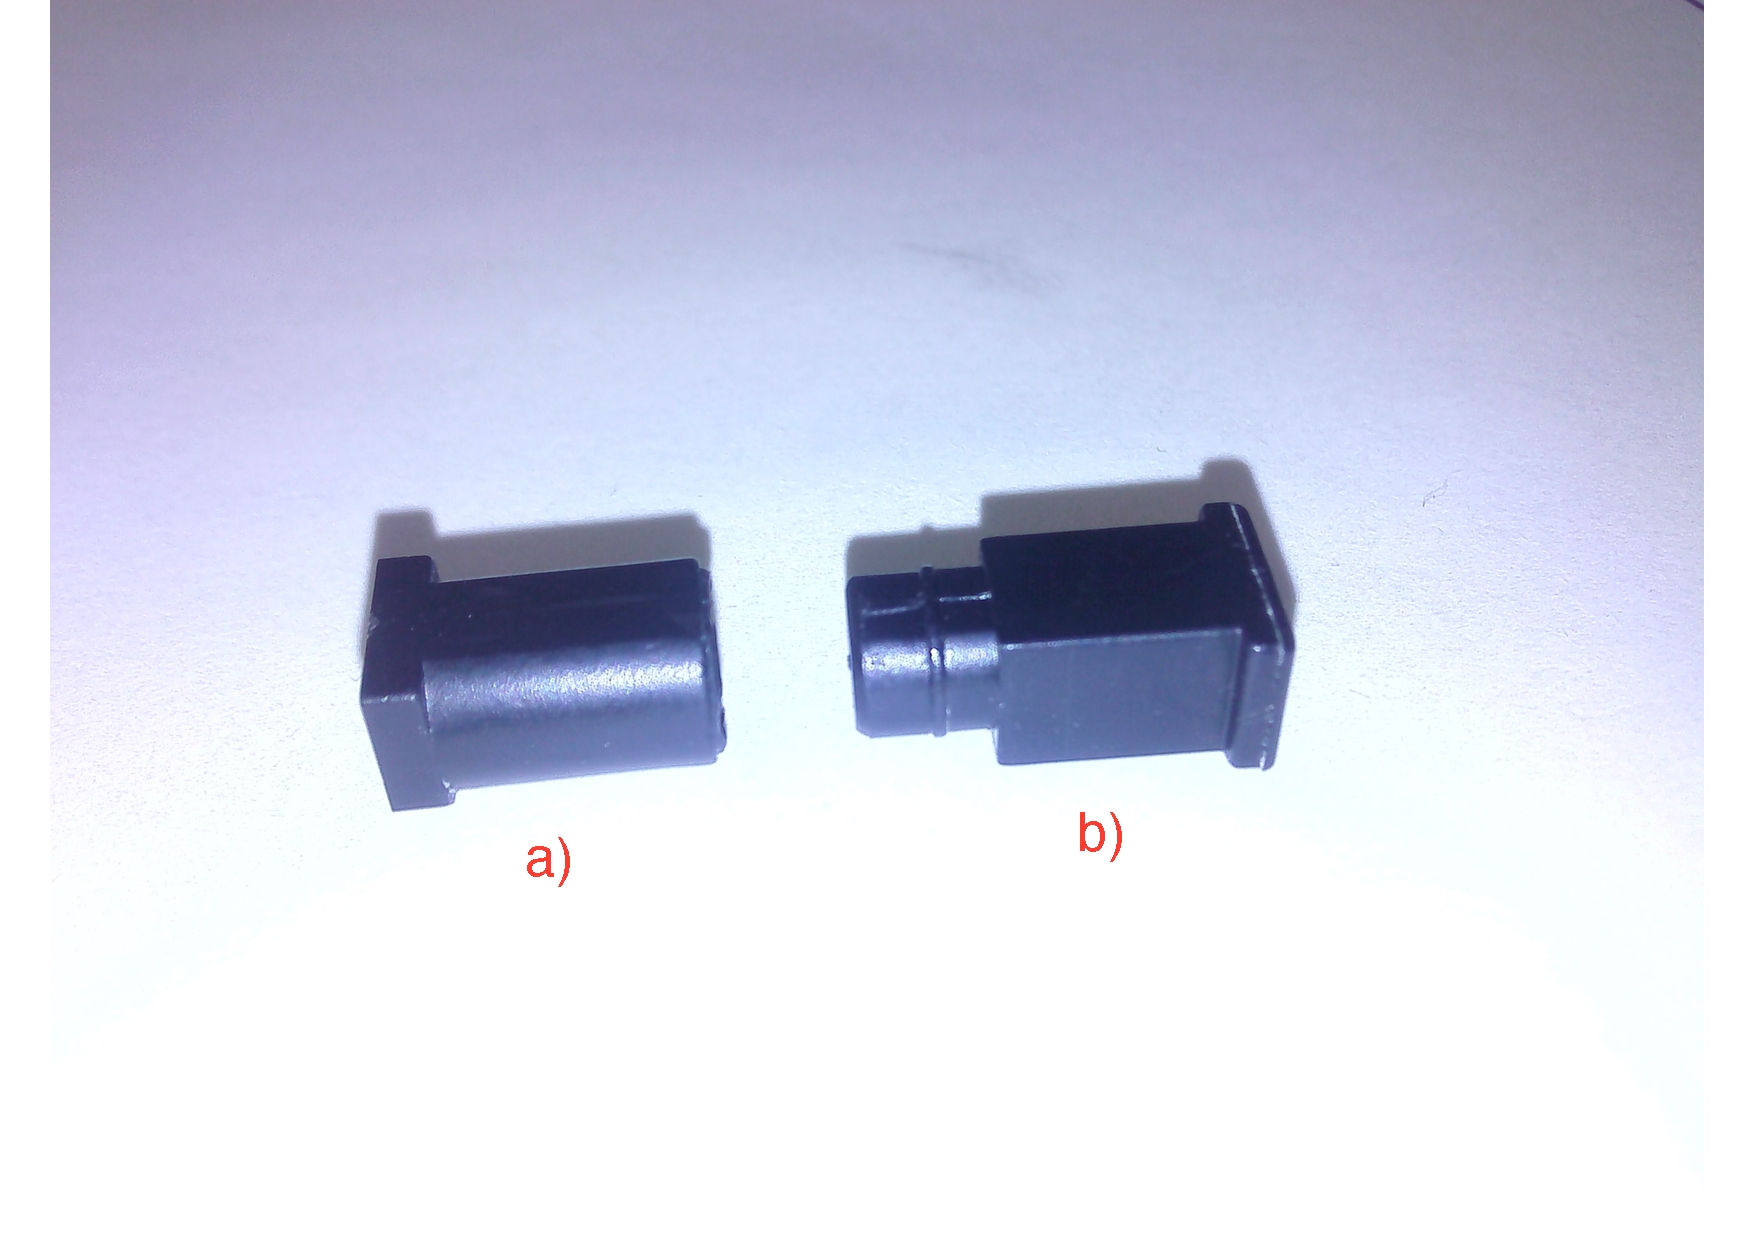
\includegraphics[width=0.8\linewidth]{fig/side_mrd_optical_con.pdf}
\end{center}
\caption{
Optical connector for the Side-MRD scintillator. a) MPPC cover. b) Ferrule.
}
\label{fig:side_mrd_optical_con}
\end{figure}

\begin{figure}[tbh]
\begin{center}
\includegraphics[width=0.8\linewidth]{fig/side_mrd_optical_scheme.pdf}
\end{center}
\caption{
Scheme of the MPPC placement in optical connector.  a) MPPC cover. b) Ferrule. c) Spring (sponge rubber). d) MPPC.
}
\label{fig:side_mrd_optical_scheme}
\end{figure}

Construction of scintillator bars of the Side-MRD modules had been completed at INR in Russia, and they were transported to Japan in July 2017. Before and after the shipping their perfomance were check with cosmic rays. The main mesured parameters were light yield and light yield assymetry. For the light yields $LY_{1}$ and $LY_{2}$ at counter's two ends correspondent assymetry is calculated as $100\% \times \frac{LY_{1}-LY_{2}}{LY_{1}+LY_{2}}$. Thus at INR we selected 324 counters from total 332 produced with mean light yield of 45 p.e./MIP and assymetry less than 10 \% at the center of the bar. When counters arrived to Japan their perfomance were checked once again at Yokohama National University. In the bench setup here two small trigger counters were put in the center of measured bars. Trigger signal is the coincidence between top and buttom trigger counters made of $NaI (Tl)$ crystals of $6 \times 6 \times 17 cm^{3}$ size. Average total light yield obtained in the central part of the scintillator slab is 40 p.e./MIP and varies from 32 to 50 p.e/MIP. (Fig. \ref{fig:side_mrd_ly} (left)). Only two counters here showed relatively high assymetry close to 25 \% as shown in Fig. \ref{fig:side_mrd_ly} (right). By such quality assurance tests of the counters we selected 320 scintillator bars to be installed in four Side-MRD modules. In addition, for four counters there were measured time resolution for single and combination of the counters. For one counter time resolution defined as uncertanty on $(T_{left}-T{right})/2$ was obtained $\sigma$ = 1ns (Upper left plot in Fig. \ref{fig:side_mrd_combi_time}). Further, for a set of $n$ counters combined time resolution will be $\frac{(T_{L}-T_{R})_{1}+(T_{L}-T_{R})_{2}+...+(T_{L}-T_{R})_{n}}{2 \times n}$. The result of combination of 2,3,4 counters is 0.79 ns, 0.66 ns and 0.68 ns accordingly (Fig. \ref{fig:side_mrd_combi_time}).  
\begin{figure}[tbh]
\begin{center}
\includegraphics[width=0.8\linewidth]{fig/side_mrd_ly.pdf}
\end{center}
\caption{
Total light yield distribution (left) and light yield assymetry (right) measured at YNU.
}
\label{fig:side_mrd_ly}
\end{figure}

\begin{figure}[tbh]
\begin{center}
\includegraphics[width=0.8\linewidth]{fig/side_mrd_combi_time.pdf}
\end{center}
\caption{
Time resolution for one (upper left) and a set of 2,3,4 Side-MRD counters.
}
\label{fig:side_mrd_combi_time}
\end{figure}
Construction of Side-MRD modules will be done from November 2017 to January 2018 at Yokohama National University, then they will be transported to J-PARC and will be installed to the B2 floor of the T2K near detector hall before staring the T2K beam in March 2018.

\section{Physics goals}
<<<<<<< HEAD
We will measure the differential cross section for the charged-current (CC) interaction on $\mathrm{H_2O}$ and Hydrocarbon(CH)).
The water-scintillator mass ratio of the WAGASCI module is as high as 4:1 and the high purity measurement
=======
We will measure the differential cross section for the charged current interaction on $\mathrm{H_2O}$ and Hydrocarbon(CH)).
The water-scintillator mass ratio of the WAGASCI module is as high as 5:1 and the high purity measurement
>>>>>>> 3990de357c3fb55cb364cabeeaca3efa3c6b1041
of the cross section on $\mathrm{H_2O}$ is possible.
One experimental option is to remove water from one of the two WAGASCI modules. 
The water-out WAGASCI module will allow to measure pure-CH target interactions with very low momentum-threshold for protons.
It will also benefit to subtract the background from interaction with scintillator in the water target measurement.
Another option is to add the T2K proton module which is fully made of plastic scintillators.
It will allow the high statistics comparison of cross section between $\mathrm{H_2O}$ and CH and also comparison
with the ND280 measurement. The actual configuration will be optimized with detailed MC simulation by 2018 Summer.

Our setup allows the measurements of inclusive and also exclusive channels such as
$1\mu$, $1\mu 1p$, 1$\mu 1\pi^\pm \mathrm{n}p$ samples, former two of which are mainly caused by the quasi-elastic and
2p2h interaction and the latter is mainly caused by resonant or coherent pion production and deep elastic scattering.
In general, an accelerator produced neutrino beam spectrum is wide and the energy reconstruction
somehow rely on the neutrino interaction model.
Therefore, recent neutrino cross section measurement results including those from T2K are given
as a flux-integrated cross section rather than cross sections as a function of the neutrino energy to avoid bias from the model.
We can provide the flux-integrated cross section.
In addition, by combining our measurements with those at ND280, model-independent extraction of the cross section
for narrow neutrino energy spread becomes possible.
This method was demonstrated in \cite{Abe:2015biq} and also proposed by the E61 (NUPRISM) experiment.

\subsection{Expected number of events}
Expected number of CC neutrino events remaining after the event selections was evaluated with simulation.
Detailes are described in Sec.~\ref{sec:mc_study}.
In neutrino-mode, 5,400, 1,100 and 3,800 events are expected for the water-in WAGASCI module, the water-out WAGASCI module and the INGRID proton module with $5\times 10^{20}$ POT.  Among 5,400 events for the water-in WAGASCI module,78~\%  are interactions on $\mathrm{H_2O}$.
In the antineutrino-mode, 2,240, 400 and 1,500 CC antineutrino events are expected for the water-in WAGASCI module, the water-out WAGASCI module and the INGRID proton module with $5\times 10^{20}$ POT. Amongh 2,240, 74~\% are interactions on $\mathrm{H_2O}$.
The wrong-sign interactions in antineutrino-mode is 561 events, but will be removed with 90~\% or higher efficiency by Baby MIND.

%Statical errors of flux integrated CC-inclusive neutrino cross section measurements on H$_{2}$O (full acceptance) and CH targets (forward acceptance)
%will be 1.5 \% and 1.6 \% with $5\times 10^{20}$ POT in the neutrino-mode.
%Statical errors of flux integrated CC-inclusive antineutrino cross section measurements on H$_{2}$O (full acceptance) and CH targets (forward acceptance)
%will be 2.4 \% and 2.5 \% with $5\times 10^{20}$ POT in the antineutrino-mode.


%Statical errors of flux integrated H$_{2}$O to CH CC-inclusive neutrino cross section ratio measurement 
%will be 3.1 \% (full acceptance) and 2.3 \% (forward acceptance) with $5\times 10^{20}$ POT in the neutrino-mode.
%Statical errors of flux integrated H$_{2}$O to CH CC-inclusive antineutrino cross section ratio measurement will be 5 \% (full acceptance) and 3.7 \% (forward acceptance) with $5\times 10^{20}$ POT in the antineutrino-mode.

\subsection{Pseudo-monochromatic beam by using different off-axis fluxes}
The off-axis method gives narrower neutrino spectrum, and the peak energy is lower for larger off-axis angle.
<<<<<<< HEAD
There still remains a high energy tail mainly due to neutrinos from Kaon decay.
The off-axis angle of the WAGASCI location is 1.5 degree and different from the ND280 2.5 degree.
Top two plots of Fig.~\ref{fig:fluxsubtfhc} show the energy spectra of fluxes and neutrino interaction events
at these two different locations.
By using the WAGASCI measurement results, the high energy tail of ND280 flux can be somehow subtracted.
The low energy part of the WAGASCI flux can be also subtracted by using the ND280 measurement.
Bottom two plots of Fig.~\ref{fig:fluxsubtfhc} demonstrate this method.
=======
There still remains high energy tail mainly due to neutrinos from Kaon decay.
The off-axis angle of the WAGASCI location is 1.5 degree and different from the ND280 2.5 degree.
Top two plots of Figure~\ref{fig:fluxsubtfhc} show the energy spectra of fluxes and neutrino interaction events
at these two different location.
The high energy tail of ND280 flux can be somehow subtraction by using the WAGASCI measurement.
The low energy part of the WAGASCI flux can be also subtracted by using the ND280 measurement.
Bottom two plots of Figure~\ref{fig:fluxsubtfhc} demonstrate this method.
>>>>>>> 3990de357c3fb55cb364cabeeaca3efa3c6b1041
We can effectively get two fluxes, from 0.2 GeV to 0.9 GeV and 0.6 GeV and 2 GeV
and measure flux-integrated cross section for these two fluxes.
It should be noted that even though the statistical errors are drawn for each energy bin for the bottom right plot of Fig.~\ref{fig:fluxsubtfhc},
measurement results will be given as an integration across energies.

\begin{figure}[tbhp]
\begin{center}
\includegraphics[width=\textwidth]{fig/fluxsubtractFHC.pdf}
\end{center}
\caption{Energy spectra obtained by using different off-axis angle fluxes.
  Top two plots show the fluxes(left) and spectra of interaction events (right) for ND280 (off-axis 2.5 degree) and WAGASCI (off-axis 1.5 degree). Bottom two plots show the fluxes (left) and spectra of interaction events (right) obtained by
  subtraction of fluxes at ND280 and WAGASCI.
  The error bar is for the statistical error and those in the bottom right plot is obtained assuming the statistical error
<<<<<<< HEAD
  for the ND280 measurement is much smaller than that of the WAGASCI experiment.
=======
  for ND280 measurement is much smaller than that of WAGASCI experiment.
>>>>>>> 3990de357c3fb55cb364cabeeaca3efa3c6b1041
}
\label{fig:fluxsubtfhc}
\end{figure}


<<<<<<< HEAD
%Statical errors of flux integrated CC-inclusive neutrino cross section measurements on H$_{2}$O (forward acceptance) and CH targets (forward acceptance) with the pseudo-monochromatic beam
%will be 2 \% and 1.9 \% with $5\times 10^{20}$ POT in the neutrino-mode.
%Statical errors of flux integrated CC-inclusive antineutrino cross section measurements on H$_{2}$O (forward acceptance) and CH targets (forward acceptance) with the pseudo-monochromatic beam
%will be 3 \% and 2.8 \% with $5\times 10^{20}$ POT in the neutrino-mode.

\subsection{Extraction of Cross sections}
The flux-integrated CC inclusive cross sections on $\mathrm{H_2O}$ and CH are calculated from the number of selected events
with background subtraction and efficiency correction
\begin{equation*}
\sigma_{CC} = \frac{N_{sel}-N_{BG}}{\phi T \epsilon},
\end{equation*}
where $N_{sel}$ is the number of selected events from the real data,
$N_{BG}$ is the number of contaminated background events,
$\phi$ is the integrated $\nu_{\mu}$ flux, $T$ is the number of target nucleons,
and $\epsilon$ is the detection efficiency for signal estimated by MC simulation.
The number of main background events is effectively estimated from side-band samples.
The CH interaction background for the $\mathrm{H_2O}$ measurement is estimated from the measurement of the Water-out WAGASCI module and/or
the proton module.
The neutrino interaction background for the antineutrino measurement is estimated from the opposite-sign interactions selected by Baby MIND.
% The $\nu_{\mu}$ CC inclusive cross sections on water and hydrocarbon are measured from the number of selected events
%in the water and hydrocarbon regions in the central detector.
% The $\nu_{\mu}$ CC inclusive cross section ration on water to hydrocarbon is measured 
% using the two results.
The dominant error for the inclusive total cross section measurement is the uncertainty of the neutrino flux, which is $\sim$9\% now and is expected to be reduced to $\sim$6\%.
Since the flux error is dominated by the normalization type error,
the flux error can be significantly reduced for the relative comparison of the $\mathrm{H_2O}$ and CH cross sections
and the relative comparison of the ND280 and WAGASCI measurements.
For example, T2K INGRID succeeded to determine the cross section ratio for CH and Fe with 3\% precision\cite{ingrid_ccinclusive}.
For the exclusive and/or differential corss section measurements, statistical error would be dominant, size of which depending on the binning.

\subsection{Subjects WAGASCI can contribute}
Recent accelerator neutrino experiments use nuclear target e.g. organic scintillator, water and iron.
So the interaction is largely affected by nuclear effects such as Fermi motion, correlated pairs of nucleons in nucleus (two particles-two holes, 2p2h), collective nuclear effects 
%calculated with Random Phase Approximation (RPA) 
and final state interactions (FSI) of secondary particles in the nuclei after the initial neutrino interactions.

The main interaction type at the T2K energy (sub GeV) is the CC quasi-elastic (CCQE) interaction with nucleons inside nucleus.
The energy is reconstructed from the lepton momentum assuming CCQE kinematics in T2K and other interactions would bias the reconstructed energy.
Figure~\ref{fig:ene_rec_bias} shows how the reconstructed energy is affected.
The 2p2h interactions mainly happen through the interaction with a correlated nucleons pair and also through the $\Delta$ resonance interaction
followed by pion-less decay.
The 2p2h interactions are observed in electron scattering experiments \cite{escattering} where the 2p2h events were observed in the gap between quasi-elastic region and pion-production region.% as shown in Fig. \ref{fig:electrono_scattering_data}.
Neutrino experiments have attempted to measure the 2p2h interactions, but so far there are only indicative results because the energy spectrum of the neutrino beam is wide and the precision of the event-by-event determination of the neutrino energy is not good nor suffered from bias.
%separation of the QE peak and the 2p2h peak is more difficult because transferred momentum (p) and energy (w) are largely affected by  neutrino energies which cannot be determined event-by-event in the wide energy spectrum of the accelerator neutrino beam.
Our measurements, when combined with ND280 measurement, will give the cross section values for narrow energy-spread fluxes
and give insight for such interactions. 
%Our model-independent narrow neutrino spectra extracted from combined analyses of our data and ND280 data are ideal for searching the 2p2h interaction because clearer separation of the QE peak and the 2p2h peak is expected.
Another efficient way to investigate the 2p2h interaction is direct measurement of proton tracks with low momentum threshold and wide acceptance.
Figure~\ref{fig:2p2h_proton_multiplicity_angle} left plot shows proton multiplicities for the CCQE events and 2p2h events.
Figure~\ref{fig:2p2h_proton_multiplicity_angle} right plot shows opening angles of two proton-tracks for the events having two protons.
The water-out WAGASCI can provide good sample for the 2p2h interaction search because its low density medium enables the detection of low momentum protons in side acceptance.
%
%\begin{figure}[tbh]
%\begin{center}
%\includegraphics[width=0.6\linewidth]{fig/escattering.pdf}
%\end{center}
%\caption{
%Comparison of inclusive $^{12}$C(e,e') cross sections and predictions of the QE-SuSAv2 model (long-dashed red line), 2p-2h MEC model (dot-dashed brown line) and inelastic-SuSAv2 model (long dot-dashed orange line) (from Ref. \cite{escattering}).
%The sum of the three contributions is represented with a solid blue line.
%The q dependence with $\omega$ is also shown (short-dashed black line.)
%}
%\label{fig:electrono_scattering_data}
%\end{figure}
%
\begin{figure}[tbhp]
=======
Statical errors of flux integrated CC-inclusive neutrino cross section measurements on H$_{2}$O (forward acceptance) and CH targets (forward acceptance) with the pseudo-monochromatic beam
will be 2 \% and 1.9 \% with $0.5\times 10^{21}$ POT in the neutrino-mode.
Statical errors of flux integrated CC-inclusive antineutrino cross section measurements on H$_{2}$O (forward acceptance) and CH targets (forward acceptance) with the pseudo-monochromatic beam
will be 3 \% and 2.8 \% with $0.5\times 10^{21}$ POT in the neutrino-mode.


\subsection{Subjects WAGASCI can contribute}
In T2K experiment, neutrinos interact with bound nucleons in relatively heavy nuclei (Carbon and Oxygen), so the cross-section is largely affected by nuclear effects.
The nuclear effects are categorized as nucleons' momentum distribution in nucleus, interactions with  correlated pairs of nucleons in nucleus (two particles-two holes, 2p2h), collective nuclear effects 
%calculated with Random Phase Approximation (RPA) 
and final state interactions (FSI) of secondary particles in the nuclei after the initial neutrino interactions.


The 2p2h interactions mainly happen through $\Delta$ resonance interactions following a pion-less decay and interactions with a correlated nucleon pair.
The 2p2h interactions are observed in electron scattering experiments \cite{escattering} where the 2p2h events observed in the gap between Quasi-Elastic region and Pion-production region as shown in Figure \ref{fig:electrono_scattering_data}.
Neutrino experiments also attempt to measure the 2p2h interactions, but separation of the QE peak and the 2p2h peak is more difficult because transferred momentum (p) and energy (w) are largely affected by  neutrino energies which cannot be determined event-by-event in the wide energy spectrum of the accelerator neutrino beam.
Our model-independent narrow neutrino spectra extracted from combined analyses of our data and ND280 data are ideal for searching the 2p2h interaction because clearer separation of the QE peak and the 2p2h peak is expected.
Another way to observe the 2p2h interaction is direct measurement of proton tracks in CC0$\pi$ sample with low detection threshold and full acceptance.
Figure \ref{fig:2p2h_proton_multiplicity_angle} shows proton multiplicities after FSI in CCQE events and 2p2h events, and Figure \ref{fig:2p2h_proton_multiplicity_angle} shows opening angles among two proton tracks in the same samples.
The water-out WAGASCI can provide good sample for the 2p2h interaction search because its low density medium enables the detection of low momentum protons in addition to the full acceptance.

\begin{figure}[tbh]
>>>>>>> 3990de357c3fb55cb364cabeeaca3efa3c6b1041
\begin{center}
\includegraphics[width=\linewidth]{fig/recE.pdf}
\end{center}
\caption{Left: reconstructed neutrino energy for CCQE and 2p2h interactions of 600~MeV muon neutrinos on $^{12}C$ simulated with a mode.
  Right: difference between true and reconstructed energy of the $\nu_e$ CCQE-like sample.
  The energy is reconstructed from the lepton momentum assuming the kinematics of the CCQE interaction.
  Both plots from \cite{Abe:2017vifw}
}
\label{fig:ene_rec_bias}
\end{figure}
%
\begin{figure}[tbhp]
 \begin{center}
  \begin{subfigure}{0.48\textwidth}
     \includegraphics[width=\linewidth]{fig/2p2h_proton_multiplicity.pdf}
    \end{subfigure}
  \begin{subfigure}{0.48\textwidth}
    \includegraphics[width=\linewidth]{fig/2p2h_proton_angle.pdf}
    \end{subfigure}    
    \end{center}
  \caption{
Proton multiplicities (left) and opening angles between two proton tracks (right) for CCQE events and 2p2h events.
The final-state interaction is taking into account.
}
\label{fig:2p2h_proton_multiplicity_angle}
\end{figure}


% The corrections from collective nuclear effects calculated by RPA as a function of $Q^{2}$ are shown in Fig. \ref{fig:effect_rpa}.
% The $Q^{2}$ dependence of the correction can be tested by measuring angular distribution of muons in CC1-$\mu$ and CC1-$\mu 1p$ events.
% The uncertainties of the corrections in low (high) $Q^{2}$ regions can be constrained by observing the events with a forward-going (high-angle) muon, so it is essential to measure muon tracks with full acceptance.
There are various models which describe the collective nuclear effects \cite{collective_nuclear_effect}.
The wide acceptance of the WAGASCI experiment will provide information complementary to ND280 and will play important role to select/tune models.
%The $Q^{2}$ dependence of the effects can be tested by measuring angular distribution of muons in CC1-$\mu$ and CC1-$\mu 1p$ events.
%The uncertainties of the effects in low (high) $Q^{2}$ regions can be constrained by observing the events with a forward-going (high-angle) muon, so it is essential to measure muon tracks with full acceptance.
% Based on the measurement, we can evaluate the models and determine model parameters.

T2K is starting to use $\nu_{e}$ CC1$\pi$ samples at the far detector to increase the statistics.
One of the biggest uncertainty of the CC1$\pi$ sample comes from the final state interactions of pions in the nuclei after the initial neutrino interactions because they change the multiplicity, charge and kinematics of the pions.
The multi-pion production events can be migrated into the CC1$\pi$ sample due to the FSIs, and they become backgrounds.
The WAGASCI module has a capability to distinguish the pion track and proton track from d$E$/d$x$, so 
WAGASCI can provide the CC1$\pi$ cross section with low momentum threshold and wide acceptance for pion tracks.
%constrain the uncertainties from the pion FSIs by measuring pion rescattering in the detector and pion multiplicity in $\nu_{\mu}$ CCn$\pi$ sample
%with low detection threshold and full acceptance for pion tracks.
%The water-out WAGASCI can provide good sample for the pion FSI studies because its low density medium enables the detection of low momentum pions in addition to the full acceptance.





\section{Status of J-PARC T59 experiment}
We had submitted a proposal of a test experiment to test a new detector with a water target, WAGASCI, at the T2K near detector hall to J-PARC PAC on April 2014, and the proposal was approved as J-PARC T59.
 There are several updates on the project after three years from then.
 Fist, the start time of neutrino beam measurement is changed from December 2015 to October 2017, and the requested neutrino beam is changed from $1\times10^{21}$ POT of $\nu$ beam to $0.8\times10^{21} $POT of anti-$\nu$ beam. 
 Second, the detector configuration is changed. In the original proposal, central neutrino detector are expected to be surrounded by newly developed muon-range detectors (MRDs), but we will use spare neutrino detectors of the T2K experiment instead of them during neutrino beam measurement from October to December 2017. Construction of the newly developed MRDs, Baby-MIND and Side-MRD, is in progress, and they will be installed to the both sides and the downstream of the central neutrino detector from January to March 2018. Then, we will resume neutrino beam measurements from March 2018 and will take the neutrino beam data until May 2018.

\subsection{Plans from October 2017 to May 2018}
J-PARC MR will extract its proton beam to T2K neutrino beam-line from October to December 2017, and, from March to May 2018. T2K experiment will produce anti-neutrino beam and will accumulate $\sim8\times10^{20}$ POT data during the above period.


 J-PARC T59 will perform neutrino beam measurements on the B2 floor of the T2K near neutrino detector hall during the above period to test basic performances of the WAGASCI detector and new electronics. During the beam measurements from October to December 2017, one WAGASCI module will be placed between spare neutrino detectors of the T2K experiment, INGRID Proton module and INGRID standard module as shown in Fig. \ref{fig:det_config_oct_dec2017}.
Detector location on the B2 floor of T2K near detector hall is shown in Fig. \ref{fig:det_loc_oct_dec2017}. Here, the INGRID Proton module is used as a charged particle VETO detector and, the INGRID standard module is used as a downstream muon detector. 
We had submitted a proposal to use these spare neutrino detectors for the T59 neutrino beam measurements to the T2K collaboration, and we got an approval from T2K. 

 \begin{figure}[tbh]
\begin{center}
\includegraphics[width=0.8\linewidth]{fig/tmp.pdf}
% \includegraphics[width=0.8\linewidth]{fig/all_detector2.pdf}
\end{center}
\caption{
J-PARC T59 detector configuration from Oct. to Dec. 2017
}
\label{fig:det_confg_oct_dec2017}
\end{figure}


\begin{figure}[tbh]
\begin{center}
\includegraphics[width=0.8\linewidth]{fig/tmp.pdf}
% \includegraphics[width=0.8\linewidth]{fig/all_detector2.pdf}
\end{center}
\caption{
J-PARC T59 detector location from Oct. to Dec. 2017
}
\label{fig:det_loc_oct_dec2017}
\end{figure}


During the beam measurements from March to May 2018, Baby-MIDN and two side muon-range detector (Side-MRD) modules will be installed on the downstream and the both sides of the WAGASCI detector, as shown in Fig. \ref{fig:det_config_mar_may2018}, to increase angular acceptance for secondary charged particles from neutrino interactions.
 
\begin{figure}[tbh]
\begin{center}
\includegraphics[width=0.8\linewidth]{fig/tmp.pdf}
% \includegraphics[width=0.8\linewidth]{fig/all_detector2.pdf}
\end{center}
\caption{
J-PARC T59 detector configuration with Baby-MIND and two Side-MRD modules from Mar. to May 2018.
}
\label{fig:det_config_mar_may2018}
\end{figure}


\section{Detector performance}
\subsection{Wagasci module}
To demonstrate the performance of the Wagasci module and also to study the neutrino interaction,
the first Wagasci module was installed at the on-axis position, in front of the T2K INGRID horizontal center module
in 2016.
The INGRID module is made of iron plates and segmented plastic scintillator bars.
It's cross sectional size viewed from the beam direction is 1~m$\times$1~m.
The charged current interactions in the Wagasci module are selected by requiring a muon track candidate
in the INGRIRD modules.
Here, we describe the performance of the Wagasci module evaluated at this T2K on-axis measurement.
Figure~\ref{fig:wmlight} shows the light yeild of channels for muons produced by the interaction of neutrinos
in the hall wall.
The light yield is sufficiently hgih to get good hit efficieincy.  
\begin{figure}[tbh]
\begin{center}
\includegraphics[width=0.5\linewidth]{fig/wmlight.pdf}
\end{center}
\caption{Light yield of channels for muons produced by the interaction of neutrinos
  in the hall wall.
}
\label{fig:wmlight}
\end{figure}
The tracking efficiency in 2-dimentional projected plane was evalualted by comparing the reconstructed track
in the Wagasci module and the INGRID module and shown in Fig.\ref{fig:wmefficiency}.
Note that that the tracking efficinecy for high angle ($>70\deg$) is not evaluated because of the acceptance
of the INGRID module, not because of the limitation of the Wagasci module.
\begin{figure}[tbh]
  \begin{center}
   \begin{subfigure}{0.48\textwidth}
     \includegraphics[width=\linewidth]{fig/wmeffvshit.pdf}
    \end{subfigure}
  \begin{subfigure}{0.48\textwidth}
      \includegraphics[width=\linewidth]{fig/wmeffvsangle.pdf}
    \end{subfigure}    
    \end{center}
  \caption{2D track reconstruction efficiency as a function of number of hits (left) and track angle (right).
  Here the track angle is the one reconstructed by the INGRID module.}
\label{fig:wmefficiency}
\end{figure}


\subsection{Baby MIND}
The Baby MIND construction was completed in June 2017, and it was then tested in June and July 2017 at the Proton Synchrotron experimental hall at CERN with a mixed particle beam comprising mostly muons whose momenta could be selected between 0.5 and 5 GeV/c. An event display from the summer 2017 tests is shown in Figure \ref{beam_vs_cosmic}.

\inserttwographs{0.45}{baby_mind_wagasci_rough_cad.png}{0.50}{baby_mind_layout.png}{Left) WAGASCI modules: flanked by 2 side muon range detectors (sMRD) and one downstream muon detector (Baby MIND). Right) side view layout of the Baby MIND during beam tests at CERN.}{wagasci-layout}


\insertgraph{1.0}{comparing_beam_cosmics.png}{Comparison of a beam muon and cosmic muon in the three different geometrical projections of the detector. The beam impinges on the detector from the left. The arrows indicate the direction of travel of these muons. The direction of the cosmic muon is inferred from timing information.}{beam_vs_cosmic}


All counters were measured at INR Moscow with a cosmic ray setup using the same type S12571-025C MPPCs and CAEN DT5742 digitizer \cite{Antonova:2017cdw}. The average light yield (sum from both ends) was measured to be 37.5 photo-electrons (p.e.) per minimum ionizing particle (MIP) and 65 p.e./MIP for vertical and horizontal counters, respectively. After shipment to CERN, all counters were tested once more individually with an LED test setup \cite{led_test_system}. 0.1\% of counters failed the LED tests and were therefore not used during the assembly of modules. 

\input{perform_smrd}
\section{MC studies}

\subsection{Detector simulation}
Expected number of neutrino events in the WAGASCI detector is evaluated with Monte Carlo simulations. 
Neutrino beam flux at the detector location is simulated by T2K neutrino flux generator, JNUBEAM, neutrino interactions with target materials are simulated by a neutrino interaction simulator, NEUT, detector responses are simulated using GEANT4-based simulation.
The neutrino flux at the detector location, 1.5 degrees away from the J-PARC neutrino beam axis, is shown in Figure \ref{fig:b2flux}, and its mean neutrino energy is around 0.68 GeV.


\subsubsection{Detector geometry}
The detector geometry in the GEANT4-based simulation is slightly different from the actual detector as shown in Fig. \ref{fig:wagasci_mc_geometry}.
The active neutrino target region consists of four WAGASCI modules, and each WAGASCI detector has the dimension with 100 cm $\times$ 100 cm in the x and y directions and 50 cm along the beam direction.
An event display of a MC event in the WAGASCI detectors is shown in Figure \ref{fig:wagasci_event_display}.
Two Side-MRD modules is installed at both sides of the WAGASCI modules, and each Side-MRD module consists of ten iron plates whose dimension is 3 cm (thickness) $\times$ 180 cm (height) $\times$ 320 cm (width). 
The distance between the Side-MRD modules and WAGASCI modules is 60 cm.
The downstream-MRD equivalent to the Baby-MIND is installed at the downstream of the WAGASCI modules.
The downstream-MRD consists of ten iron plates whose dimension is  3 cm (thickness) $\times$ 180 cm (height) $\times$ 320 cm (width) and another ten iron plates whose dimension is 6 cm (thickness) $\times$ 180 cm (height) $\times$ 320 cm (width).
The distance between the downstream-MRD modules and WAGASCI modules is 60 cm.

\begin{figure}[tbh]
\begin{center}
\includegraphics[width=0.8\linewidth]{fig/wagasci_mc_geometry.pdf}
% \includegraphics[width=0.8\linewidth]{fig/all_detector2.pdf}
\end{center}
\caption{
Geometry of the detectors in the Monte Carlo simulation.}
\label{fig:wagasci_mc_geometry}
\end{figure}

\begin{figure}[tbh]
\begin{center}
\includegraphics[width=0.8\linewidth]{fig/wagasci_event_display.pdf}
% \includegraphics[width=0.8\linewidth]{fig/all_detector2.pdf}
\end{center}
\caption{
An event display of MC event in WAGASCI detectors. Green lines are scintillators and red circles are the hit channels.}
\label{fig:wagasci_mc_geometry}
\end{figure}

In order to estimate backgrounds from neutrino interactions in the wall and floor of the experimental hall, the geometry of the experimental hall is implemented in the GEANT4-based detector simulation.


\subsubsection{Response of detector components}
The energy deposit inside the scintillator is converted into the number of photons. 
The effects of collection and attenuation of the light in the scintillator and the WLS fiber are simulated, and the MPPC response is also taken into account. 
The light yield is smeared according to statistical fluctuations and electrical noise.


\subsection{Track reconstruction}
To select neutrino interaction from the hit patterns, a track reconstruction algorithm is developed.
The flow of the track reconstruction is as follows.
\begin{enumerate}
\item Two-dimensional track reconstruction in each sub-detectors
\item Track matching among the sub-detectors
\item Three -dimensional track reconstruction
\end{enumerate}

Add explanation about two-dim reco, track matching and three-dim reco here.


\subsection{Event selection}

\subsubsection{Vertexing}


\subsubsection{Short track search}


\subsubsection{Fiducial volume cut}
The events with the track which starts in 5 cm from the wall of the WAGASCI module are rejected to remove the background from the outside as shown in Fig. \ref{fig:fv_cut}.

\begin{figure}[tbh]
  \begin{center}
   \begin{subfigure}{0.48\textwidth}
     \includegraphics[width=\linewidth]{fig/fv_cut_y.pdf}
    \end{subfigure}
  \begin{subfigure}{0.48\textwidth}
      \includegraphics[width=\linewidth]{fig/fv_cut_z.pdf}
    \end{subfigure}    
    \end{center}
  \caption{Event selection with the vertex of the track.
Blue hist. are events from the WAGASCI modules, green hist. are events from the experimental hall, and yellow hist. are events from the Side-MRD modules and the downstream-MRD.
}
\label{fig:fv_cut}
\end{figure}


\subsubsection{Penetrated iron plates cut}


\begin{figure}[tbh]
  \begin{center}
   \begin{subfigure}{0.48\textwidth}
     \includegraphics[width=\linewidth]{fig/penetrated_iron_plates_cut_sidemrd.pdf}
    \end{subfigure}
  \begin{subfigure}{0.48\textwidth}
      \includegraphics[width=\linewidth]{fig/penetrated_iron_plates_cut_babymind.pdf}
    \end{subfigure}    
    \end{center}
  \caption{
Event selection with the number of the penetrated iron plates in the Side-MRD modules (left) and the Baby-MIIND (right).
Blue and red hist. are events from the WAGASCI modules, green hist. are events from the experimental hall, and yellow hist. are events from the Side-MRD modules and the Baby-MIND.
}
\label{fig:penetrated_iron_plates_cut}
\end{figure}







%\input{organization.tex}
\section{Schedule}
We would like to start a physics data taking from T2K beam time after the summer shutdown in 2018.
By then, commissioning and tests of the detectors will be completed in J-PARC T59.
The experiment can run parasitically with T2K, therefore we request no dedicated beam time nor beam condition as discussed in the following section.





Once the approved POT is accumulated, the WAGASCI modules will be removed from the experimental site, but we would like to keep the Baby-MIND and the Side-MRD modules on the B2 floor of the NM pit as common platforms of future neutrino experiments using the T2K neutrino beam.

\section{Requests}
\subsection{Beam condition and beam time}
The experiment can run parasitically with T2K, therefore we request no dedicated beam time nor beam condition.
We request \textcolor{red}{$1 \times 10^{21}$ POT neutrino beam data and another $1 \times 10^{21}$ POT antineutrino data}.
% Assuming 250kW beam operation, it corresponds to $\sim$ 100 days of data taking.

\subsection{Request of equipment}
\begin{itemize}
\item Site in the B2 floor of the near detector hall (Fig. \ref{fig:location})
\item Electricity \textcolor{red}{($\sim$10kW)} for the electronics and water circulation system
\item Beam timing signal and spill information
\item Network connection
\end{itemize}

\input{conclusion.tex}

\end{document}  
